\chapter{Software-Qualität}
\label{ch:software-qualitaet}

Um sicherzustellen, dass Software erwartungsgemäß funktioniert und eine Weiterentwicklung vereinfacht wird, ergibt es
Sinn, verschiedene Aspekte zu berücksichtigen, die für eine verbesserte Qualität der Software sorgen.
Die Wartbarkeit der Anwendung wird in \Kapitel{sec:erweiterbarkeit} noch genauer betrachtet.

\section{Architektur der Software}
\label{sec:software-architektur}

Beim Aufbau der Software haben wir uns für eine dreischichtige Architektur und den Einsatz des \ac{MVC}-Patterns
entschieden.
Die Architektur ist in \Abbildung{fig:schichtenarchitektur} dargestellt und beinhaltet neben der Schicht zur Anzeige
des Spiels in einer Oberfläche die Logik-Schicht, in der \ua implementiert wurde, wie ein Spiel abläuft, wie
die Daten zur Kommunikation mit dem Server übersetzt werden können und auch wie die \ac{KI}s funktionieren sollen.
Im Prinzip wird hier das Zusammenspiel der Klassen aus dem Modell umgesetzt.
Die Modell-Schicht stellt die letzte und unterste Schicht dar und bietet die Klassen zur Datenhaltung und deren interne
Logik an. \\

\begin{figure}[htb]
\centering
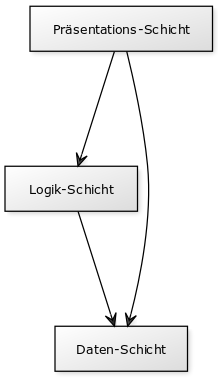
\includegraphics[width=4cm]{Bilder/Diagramm_Schichtenmodell.png}
\caption{Schichtenarchitektur der Software}
\label{fig:schichtenarchitektur}
\end{figure}

Ein wichtiger Aspekt ist hierbei, dass ein Zugriff nur auf eine untere Schicht erlaubt ist.
Somit soll verhindert werden, dass die Logik-Schicht \bspw abhängig von der Art der Darstellung ist. \\

\subsection{Package-Struktur}
\label{subsec:package-struktur}

Aufbauend darauf haben wir das \ac{MVC}-Pattern umgesetzt und dies in dem Aufbau der Package-Struktur verdeutlicht,
welche auch in \Abbildung{fig:package-struktur} zu sehen ist.
Das View-Package stellt in der Schichten-Architektur die Präsentations-Schicht dar und beinhaltet Klassen, die sich um
die Anzeige kümmern.
Dabei ist, wie das Schichtenmodell erlaubt wird, ein Zugriff auf das Modell möglich.
Die Logik-Schicht wird zum einen Teil durch das Controller-Package realisiert, in welchem insbesondere die Verknüpfung
zwischen der Geschäftslogik und der Oberfläche geschieht.
Die eigentliche Logik befindet sich dann im Service-Package, welches sich in der gleichen Schicht befindet.
Allerdings soll ein Zugriff aus Service nach Controller unterbunden werden.
Es handelt sich um eine Erweiterung des klassischen MVC-Patterns.
Zuletzt bildet das Modell-Package die oben beschriebene Modell-Schicht ab.

\begin{figure}[htb]
\centering
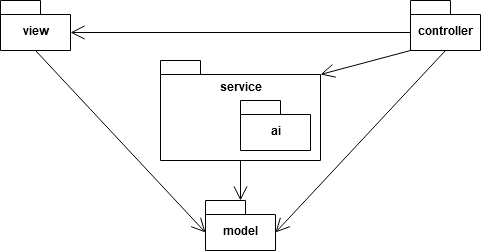
\includegraphics[width=0.6\textwidth]{Bilder/Diagramm_Paketstruktur.png}
\caption{Package-Struktur des Projekts}
\label{fig:package-struktur}
\end{figure}

\section{Automatisierte Tests}
\label{sec:tests}

Zur Sicherstellung der Korrektheit der Software wurden automatisierte Tests implementiert.
Diese dienen während der Implementierung dazu, ein gewünschtes Szenario abzubilden und anschließend den Code so zu
implementieren, dass der Test erfolgreich durchläuft.
Anschließend ist eine Refaktorisierung möglich, \dasheisst der Code wird verändert, die Funktionalität soll aber gleich
bleiben.
Ein Beispiel dafür kann eine Verbesserung der Lesbarkeit oder Wartbarkeit durch eine Auslagerung einer großen in
mehrere kleinere Methoden sein.
Diesen testgetriebenen Ansatz haben wir zwar nicht für alle Komponenten verwendet, an einigen Stellen war dies aber
durchaus hilfreich. \\

Ein weiterer Vorteil von automatisierten Tests ist, dass bei einer Weiterentwicklung sichergestellt werden kann, dass
durch eine Änderung keine ungewollten Nebeneffekte eintreten, sondern der Entwickler sicher sein kann, dass bei erfolgreich durchgelaufenen
Tests alles weiterhin funktioniert. \\

Ein Beispiel für einen Test ist in \Listing{lst:beispiel_unitttest} zu sehen.
Grundsätzlich folgt der Ausbau eines Testfalls den drei Schritten Arrange, Act und Assert.
Im ersten Schritt wird der Testfall also vorbereitet, anschließend der zu testende Use-Case aufgerufen und abschließend
geprüft, ob das gewünschte Resultat erzielt wurde.

\lstinputlisting[label=lst:beispiel_unitttest,language=Python,caption=Beispiel für einen Unit-Test]
{./Dokumente/beispiel-unittest.txt}

\section{Coding Conventions}
\label{sec:code-conventions}

Um sicherzustellen, dass der Code unabhängig vom Autor einheitlich und wartbar aufgebaut ist, wurde auf die Einhaltung
von Konventionen beim Schreiben von Quell-Code beachtet.
Viele solcher Vorgabe werden bereits durch die Programmiersprache geliefert und können daher automatisch überprüft
werden.
Dabei war Pylint als Tool hilfreich, das sich als Plugin direkt in PyCharm-IDE von JetBrains integrieren ließ und somit
bereits bei der Arbeit am Code unmittelbar Verbesserungsvorschläge macht.
Außerdem wurde in einem automatischen Prozess, der nachfolgend noch in \Kapitel{sec:github-actions} beschrieben wird,
das Tool Flake8 eingesetzt, sodass eine Überprüfung durch zwei verschiedene Programme erfolgte. \\

Darüber hinaus haben wir auch eigene Punkte abgesprochen.
Dazu zählt \bspw, dass wir bei Parametern und dem Rückgabewert an Methoden die jeweilige Typangabe ergänzt haben, obwohl
dies in Python optional ist.
Der Vorteil, der sich daraus ergeben hat, war eine bessere Unterstützung bei der Autovervollständigung und Anzeige
von möglichen Fehlern durch die IDE\@.
Darüber hinaus wurde insbesondere für die Dokumentation des Codes mit Hilfe von Docstrings der Python-Styleguide von
Google \Vgl{google-pyguide} verwendet.
Dieser beschreibt unter anderem, dass alle öffentlich sichtbaren und nicht trivialen Methoden sowie alle Klassen
dokumentiert werden sollen und gibt vor, wie die Formatierung dieses Strings auszusehen hat.
Durch den oben beschriebenen Einsatz von Pylint wurden automatisiert viele Konventionen aus diesem Styleguide überprüft,
die über die Code-Dokumentation hinausgehen.
